\section{Sensor Quality Assessment}
\label{sec:QA}

\subsection{Full-Wafer Leakage Current}
\label{subsec:QA_Itot}

\begin{figure}
	\captionsetup[subfigure]{aboveskip=-1pt,belowskip=-1pt}
	\centering
	\begin{subfigure}[b]{0.49\textwidth}
		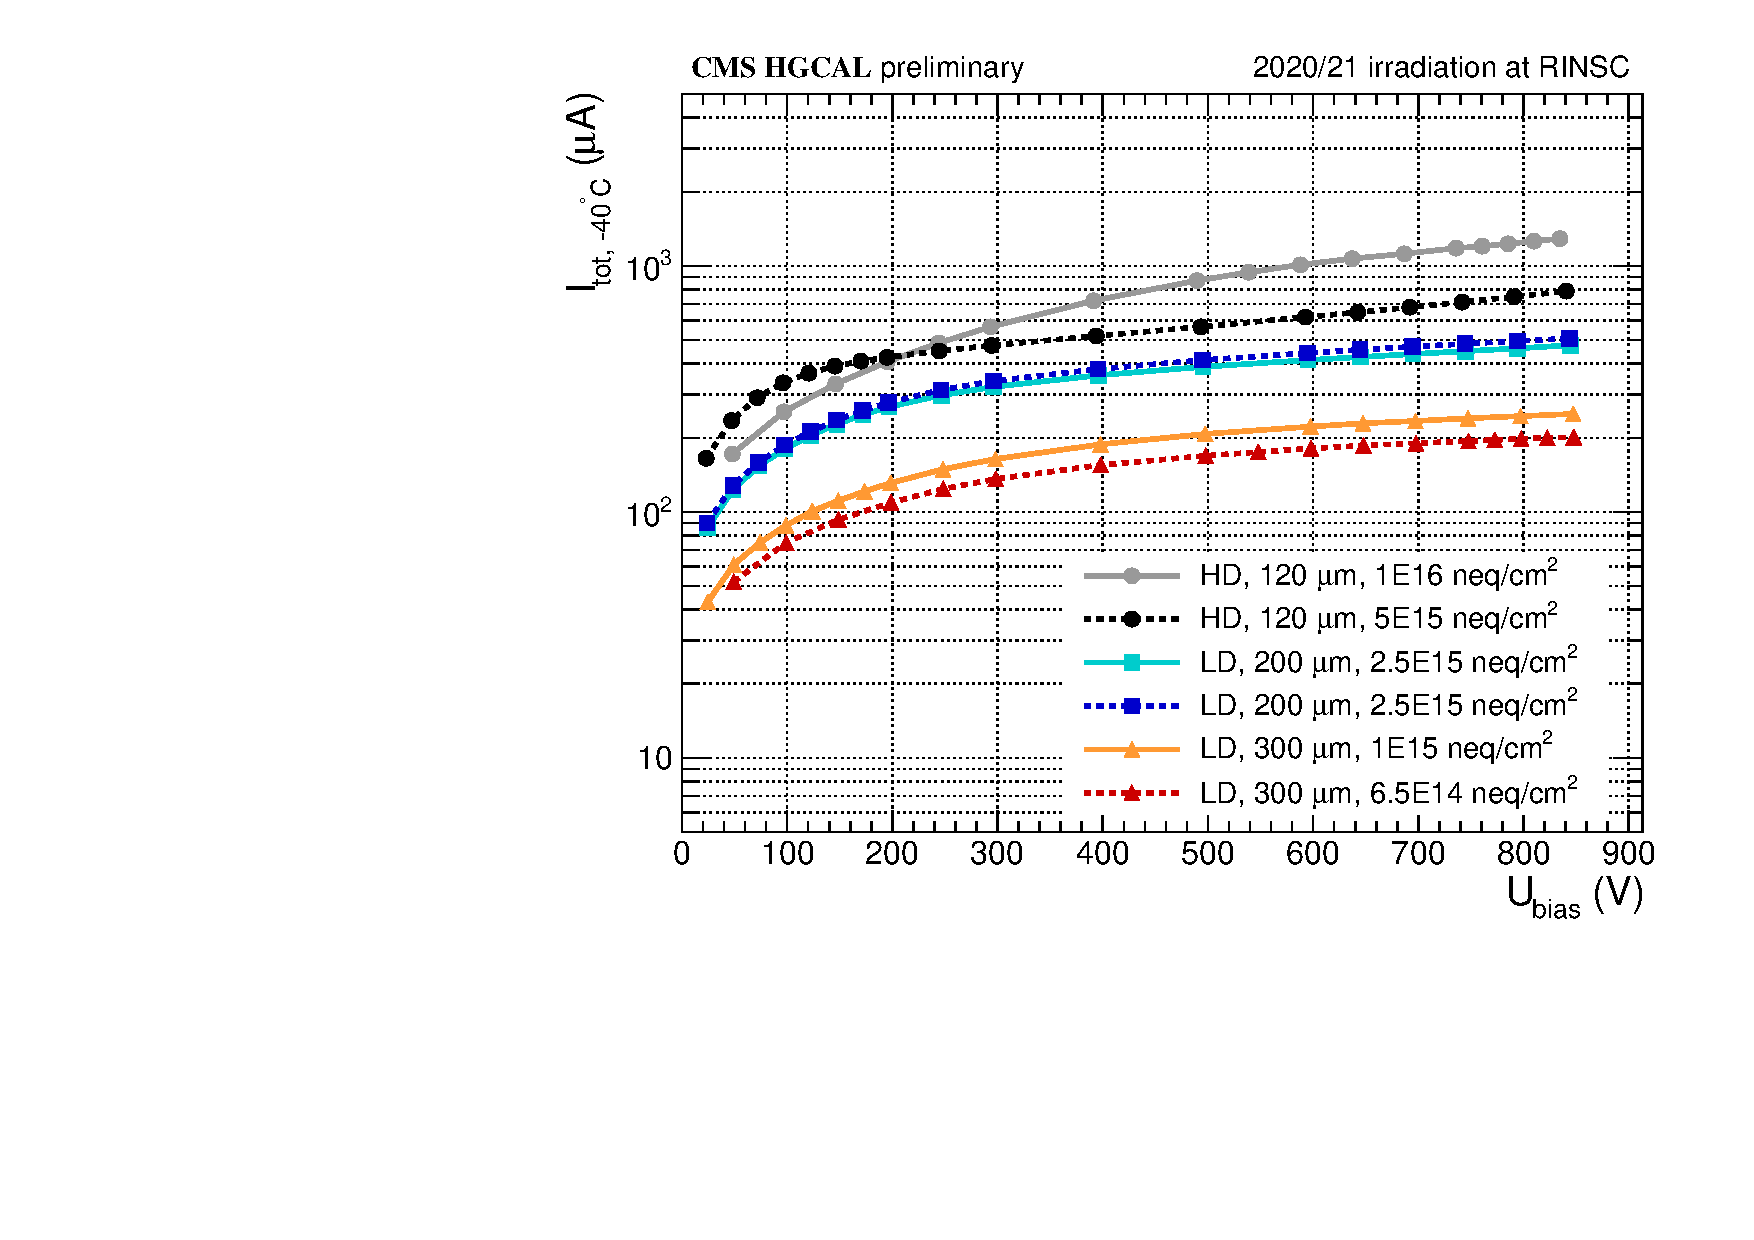
\includegraphics[width=0.999\textwidth]{plots/total_iv/total_current_IV.pdf}
		\subcaption{
		}
		\label{plot:tot_IV_good}
	\end{subfigure}
	\hfill
	\begin{subfigure}[b]{0.49\textwidth}
		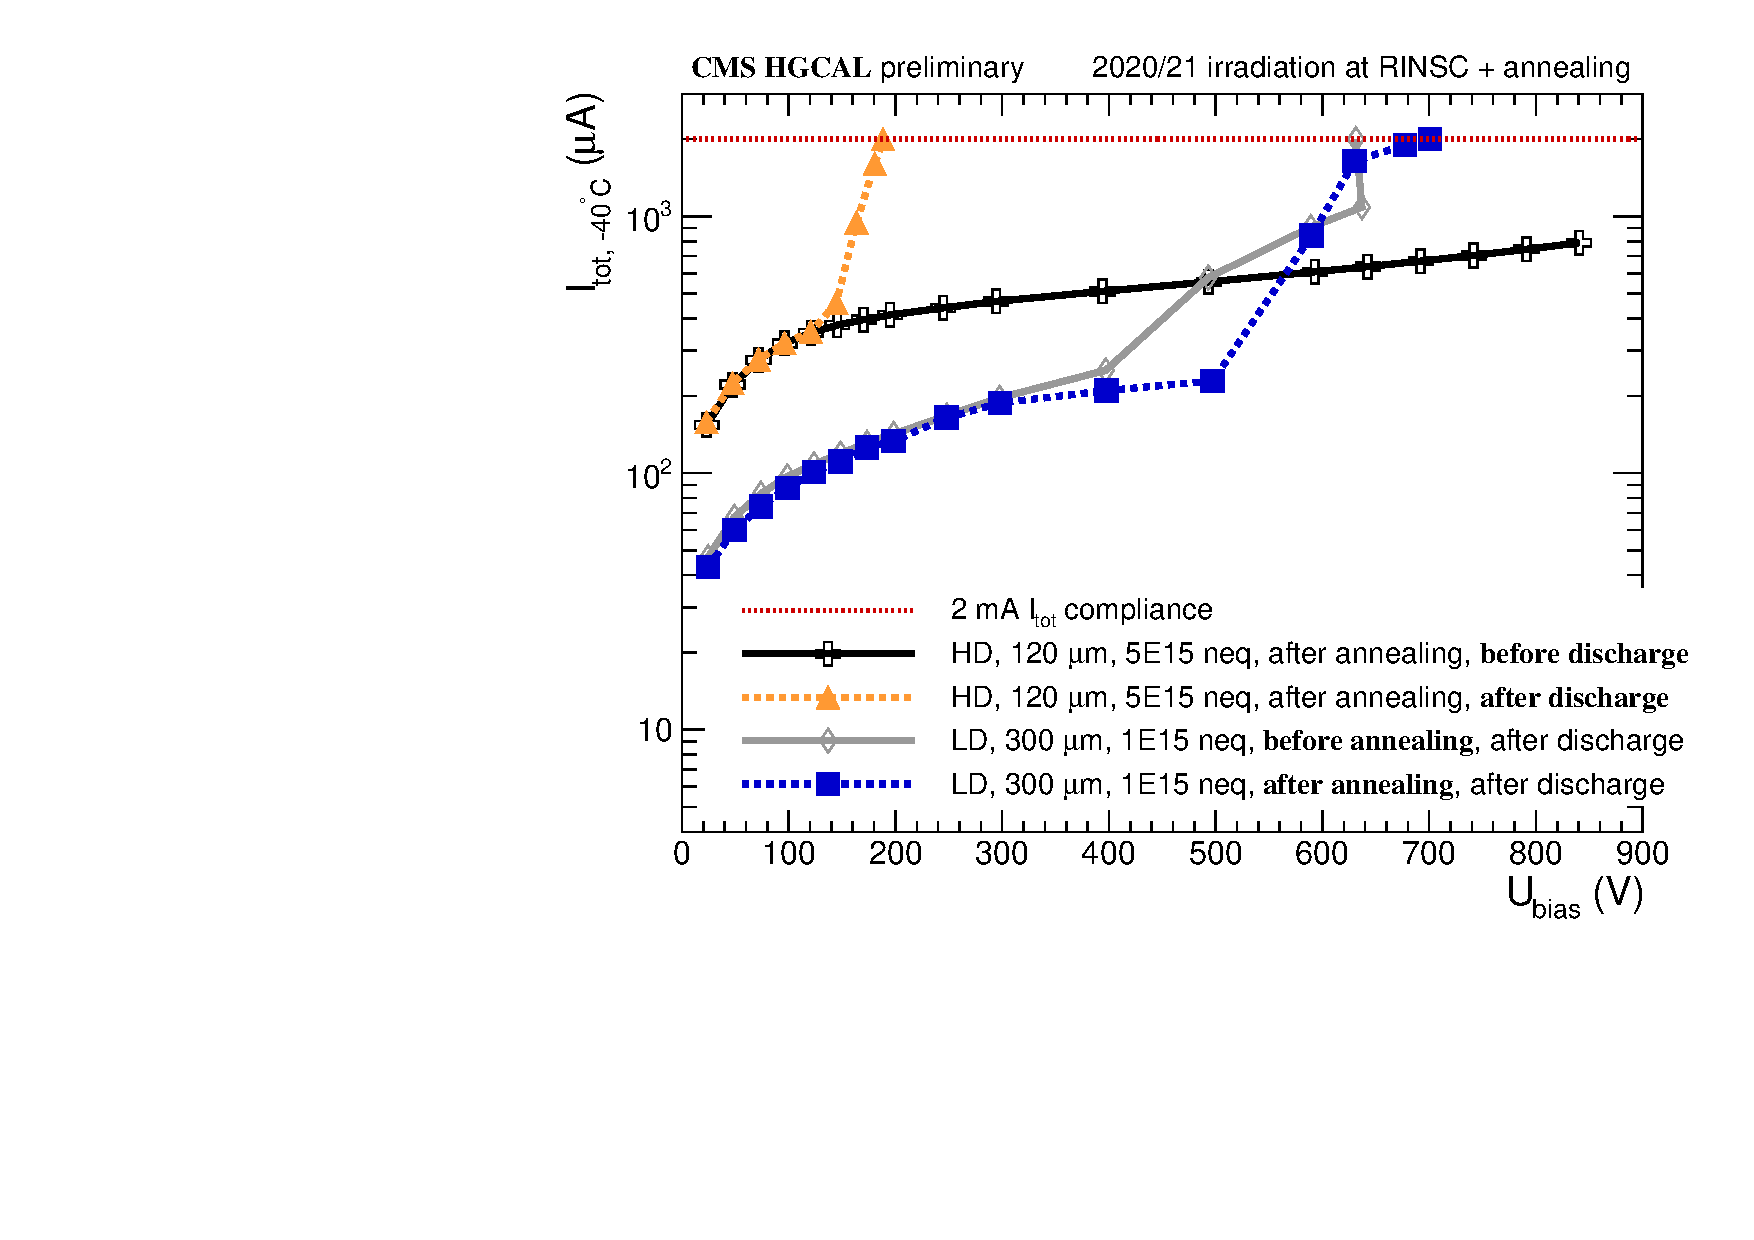
\includegraphics[width=0.999\textwidth]{plots/total_iv/total_current_IV_bad.pdf}
		\subcaption{
		}
		\label{plot:tot_IV_bad}
	\end{subfigure}
	\caption{
		(a) Full-wafer leakage currents at different effective bias voltages (a) for six good sensors from all irradiation rounds, and (b) for bad sensors with sudden leakage current increase.
	}
\end{figure}


\subsection{Per-Pad Leakage Currents}
\label{subsec:QA_Ipad}

\subsection{Per-Pad Capacitance and Depletion Voltage}
\label{subsec:QA_Vdep}
